\documentclass[a4paper, 11pt]{article}
\usepackage{comment} % enables the use of multi-line comments (\ifx \fi) 
\usepackage{lipsum} %This package just generates Lorem Ipsum filler text. 
\usepackage{fullpage} % changes the margin
\usepackage[a4paper, total={7.1in, 10in}]{geometry}
\usepackage[fleqn]{amsmath}
\usepackage{amssymb,amsthm,amsmath}
\newtheorem{theorem}{Theorem}
\newtheorem{corollary}{Corollary}
\usepackage{graphicx}
\usepackage{tikz}
\usetikzlibrary{arrows}
\usepackage{verbatim}
\usepackage[numbered]{mcode}
\usepackage{float}
\usepackage{tikz}
    \usetikzlibrary{shapes,arrows}
    \usetikzlibrary{arrows,calc,positioning}

    \tikzset{
        block/.style = {draw, rectangle,
            minimum height=1cm,
            minimum width=1.5cm},
        input/.style = {coordinate,node distance=1cm},
        output/.style = {coordinate,node distance=4cm},
        arrow/.style={draw, -latex,node distance=2cm},
        pinstyle/.style = {pin edge={latex-, black,node distance=2cm}},
        sum/.style = {draw, circle, node distance=1cm},
    }
\usepackage{xcolor}
\usepackage{mdframed}
\usepackage[shortlabels]{enumitem}
\usepackage{indentfirst}
\usepackage{hyperref}

\definecolor{question_blue}{RGB}{31,72,125}
    
\renewcommand{\thesubsection}{\thesection.\alph{subsection}}

\newenvironment{problem}[3][Problem]
    { \begin{mdframed}[backgroundcolor=gray!20] \textbf{#1 #2} \textit{(#3 points)} }
    {  \end{mdframed}}

% Define solution environment
\newenvironment{solution}
    {\textbf{Solution:}}
    {}
    
\begin{document}
\noindent
\large Haotian Fu \hfill Student ID: 520021910012    \\
Assignment 5 \hfill Instructor: Dr. Mateusz Krzyzosiak \\

\noindent\rule{7.1in}{2.8pt}
\vspace{0.5mm}

%%%%%%%%%%%%%%%%%%%%%%%%%%%%%%%%%%%%%%%%%%%%%%%%%%%%%%%%%%%%%%%%%%%%%%%%%%%%%%%%%%%%%%%%%%%%%%%%%%%%%%%%%%%%%%%%%%%%%%%%%%%%%%%%%%%%%%%%
% Problem 1
%%%%%%%%%%%%%%%%%%%%%%%%%%%%%%%%%%%%%%%%%%%%%%%%%%%%%%%%%%%%%%%%%%%%%%%%%%%%%%%%%%%%%%%%%%%%%%%%%%%%%%%%%%%%%%%%%%%%%%%%%%%%%%%%%%%%%%%%
\begin{problem}{1}{3}
\par Two conducting wires in the shape of cylinders of the same cross-sectional area, at 0 $^\circ C$ have resistivities $\rho_{01}$, $\rho_{02}$ and temperature coefficients of resistivity $\alpha_1$ and $\alpha_2$, respectively. What is the effective temperature coefficient of resistivity if the conductors are connected (a) in series, (b) in parallel.
\end{problem}
\vspace{3mm}
\begin{solution}
	\par We may as well assume both the two conducting wires have the same length. Then we denote their resistance
	\begin{align*}
		R_1 & = \rho_{1} \frac{L}{A} \\
		R_2 & = \rho_{2} \frac{L}{A}
	\end{align*}

	Then for \textbf{series}, the cross-sectional area will not change but the length doubles.
	\begin{align*}
		R_s = \rho_s \frac{2L}{A} = R_1 + R_2
	\end{align*}

	Hence
	\begin{align}
		\label{series}
		\rho_s = \frac{\rho_{1} + \rho_{2}}{2}
	\end{align}

	For \textbf{parallel}, the length will not change but the cross-sectional area doubles.
	\begin{align*}
		R_p = \rho_p \frac{L}{2A} = \frac{R_1R_2}{R_1+R_2}
	\end{align*}

	Hence
	\begin{align}
		\rho_p = \frac{2\rho_{1}\rho_{2}}{\rho_{1} + \rho_{2}}
	\end{align}

	While we know
	\begin{align}
		\rho_i = \rho_{0i}(1 + \alpha_i(T - T_0)) \qquad \text{where } i = 1,2
	\end{align}

	Namely
	\begin{align*}
		 & \rho_{0s}(1+\alpha_s(T-T_0)) = \frac{\rho_{01} + \rho_{02}}{2}(1+\alpha_s(T-T_0)) = \frac{\rho_{01}(1+\alpha_1(T-T_0)) + \rho_{02}(1+\alpha_2(T-T_0))}{2}                                        \\
		 & \frac{2\rho_{01}\rho_{02}}{\rho_{01}+\rho_{02}}(1+\alpha_p(T-T_0)) = \frac{2\rho_{01}(1+\alpha_1(T-T_0))\rho_{02}(1+\alpha_2(T-T_0))}{\rho_{01}(1+\alpha_1(T-T_0))+\rho_{02}(1+\alpha_2(T-T_0))}
	\end{align*}

	while $T_0 = 0$,hence
	\begin{align}
		\alpha_s & = \frac{\rho_{01}\alpha_1 + \rho_{02}\alpha_2}{\rho_{01} + \rho_{02}}                                                                                            \\
		\alpha_p & = \frac{\rho_{01}\alpha_2+\rho_{02}\alpha_1+(\rho_{01}+\rho_{02})\alpha_1\alpha_2(T-T_0)}{\rho_{01}+\rho_{02}+\rho_{01}\alpha_1(T-T_0)+\rho_{02}\alpha_2(T-T_0)}
		= \frac{\rho_{01}\alpha_2+\rho_{02}\alpha_1+(\rho_{01}+\rho_{02})\alpha_1\alpha_2T}{\rho_{01}+\rho_{02}+\rho_{01}\alpha_1T+\rho_{02}\alpha_2T}
	\end{align}

\end{solution}

\noindent\rule{7.1in}{2.8pt}

%%%%%%%%%%%%%%%%%%%%%%%%%%%%%%%%%%%%%%%%%%%%%%%%%%%%%%%%%%%%%%%%%%%%%%%%%%%%%%%%%%%%%%%%%%%%%%%%%%%%%%%%%%%%%%%%%%%%%%%%%%%%%%%%%%%%%%%%
% Problem 2
%%%%%%%%%%%%%%%%%%%%%%%%%%%%%%%%%%%%%%%%%%%%%%%%%%%%%%%%%%%%%%%%%%%%%%%%%%%%%%%%%%%%%%%%%%%%%%%%%%%%%%%%%%%%%%%%%%%%%%%%%%%%%%%%%%%%%%%%
\begin{problem}{2}{4}
\par For the system of resistors shown in the figure, find the equivalent resistance between points $A$ and $B$.
\end{problem}
\begin{figure}[!htbp]
	\centering
	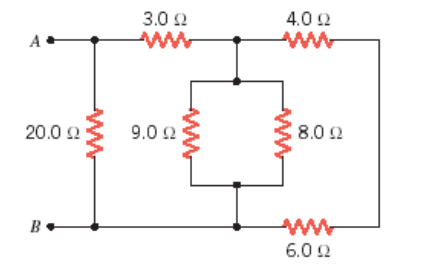
\includegraphics[width=0.3\textwidth]{hw5_p2_question.png}
	\label{fig:p2}
\end{figure}

\begin{solution}
	\par We first analyze the circuit diagram as follows.
	\begin{figure}[!htbp]
		\centering
		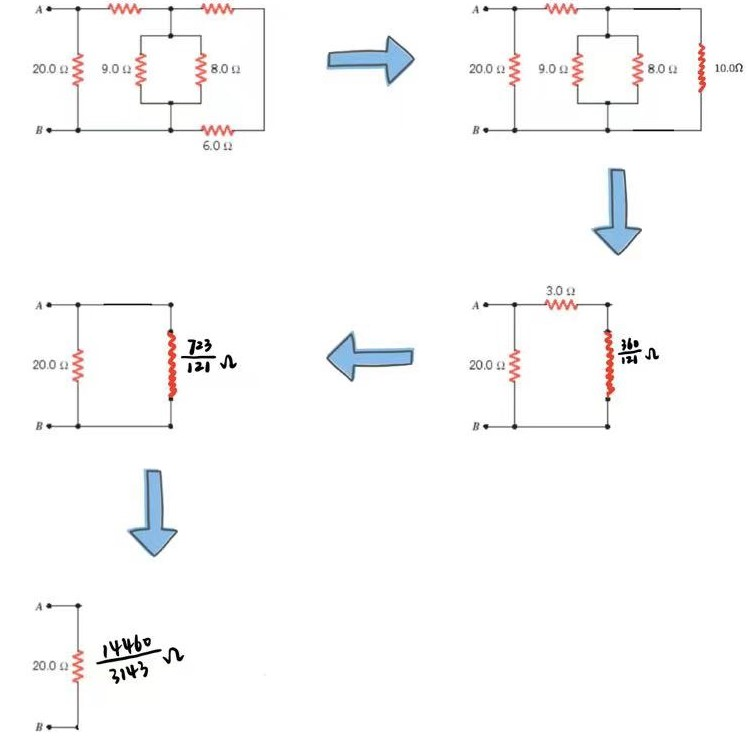
\includegraphics[width=0.5\textwidth]{hw5_p2_circuit.jpg}
		\caption{Analysis Process}
		\label{fig:circuit}
	\end{figure}

	As the diagram shows, we calculate the parallel resistance with $4\Omega$ and $6\Omega$ being a series first.
	\begin{align*}
		R_{p} = \frac{1}{\frac{1}{9}+\frac{1}{8}+\frac{1}{4+6}} = \frac{360}{121}\ [\Omega]
	\end{align*}

	Then calculate the series
	\begin{align*}
		R_{s} = 3 + \frac{360}{121} = \frac{723}{121} \ [\Omega]
	\end{align*}

	At last calculate the \textbf{equivalent resistance}
	\begin{align}
		R_{eq} = \frac{1}{\frac{1}{20}+\frac{1}{723/121}} = \frac{14460}{3143}\ [\Omega]
	\end{align}
\end{solution}

\noindent\rule{7.1in}{2.8pt}

%%%%%%%%%%%%%%%%%%%%%%%%%%%%%%%%%%%%%%%%%%%%%%%%%%%%%%%%%%%%%%%%%%%%%%%%%%%%%%%%%%%%%%%%%%%%%%%%%%%%%%%%%%%%%%%%%%%%%%%%%%%%%%%%%%%%%%%%
% Problem 3
%%%%%%%%%%%%%%%%%%%%%%%%%%%%%%%%%%%%%%%%%%%%%%%%%%%%%%%%%%%%%%%%%%%%%%%%%%%%%%%%%%%%%%%%%%%%%%%%%%%%%%%%%%%%%%%%%%%%%%%%%%%%%%%%%%%%%%%%
\begin{problem}{3}{4}
\par Twelve identical resistors, each of resistance $R$, are connected to form a cube-shaped circuit (see the figure). Find the equivalent resistance  between points $A$ and $B$. \\
\textit{Hint: Use symmetry.}
\end{problem}
\begin{figure}[!htbp]
	\centering
	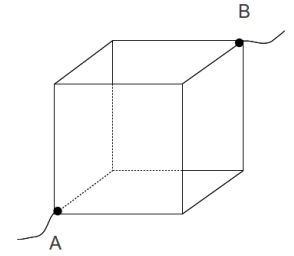
\includegraphics[width=0.4\textwidth]{hw5_p3_question.png}
	\label{fig:p3}
\end{figure}

\begin{solution}
	\par We may first consider the symmetry to divide the cube into three parts as follows.
	\begin{figure}[!htbp]
		\centering
		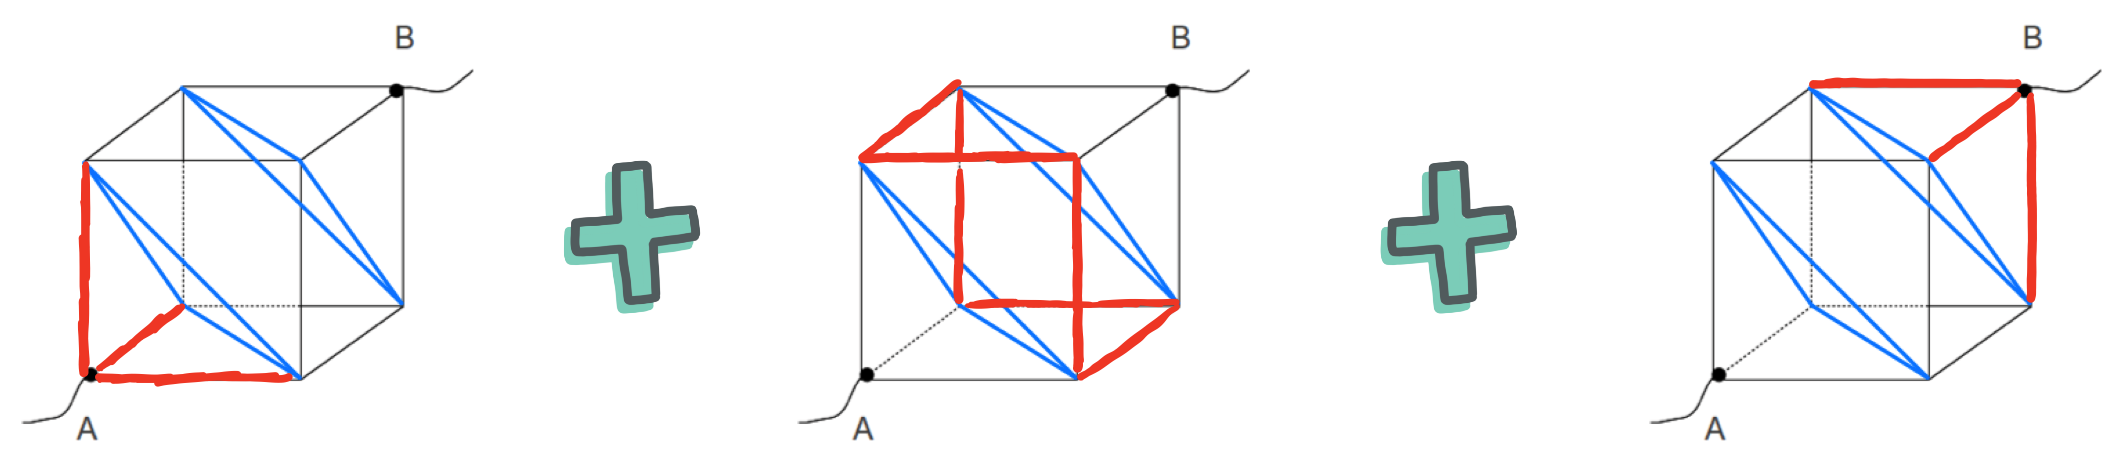
\includegraphics[width=0.5\textwidth]{hw5_p3_analysis.png}
		\caption{Symmetry Analysis}
	\end{figure}

	Apparently, it is equivalent to three resistors in serires which are all composed of parallel resistors, shown as follows.
	\begin{figure}[!htbp]
		\centering
		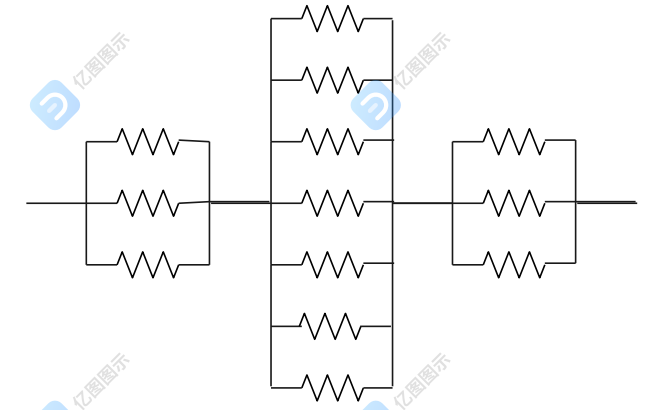
\includegraphics[width=0.4\textwidth]{hw5_p3_circuit.png}
		\caption{Equivalent Circuit}
	\end{figure}

	We then calculate the equivalent resistance separately. \\
	For the left side
	\begin{align*}
		R_{left} = \frac{R}{3}
	\end{align*}
	For the middle part
	\begin{align*}
		R_{middle} = \frac{R}{6}
	\end{align*}
	For the right side
	\begin{align*}
		R_{right} = \frac{R}{3}
	\end{align*}

	Hence the total equivalent resistance is
	\begin{align}
		R_{eq} = \frac{5R}{6}
	\end{align}
\end{solution}

\noindent\rule{7.1in}{2.8pt}

%%%%%%%%%%%%%%%%%%%%%%%%%%%%%%%%%%%%%%%%%%%%%%%%%%%%%%%%%%%%%%%%%%%%%%%%%%%%%%%%%%%%%%%%%%%%%%%%%%%%%%%%%%%%%%%%%%%%%%%%%%%%%%%%%%%%%%%%
% Problem 4
%%%%%%%%%%%%%%%%%%%%%%%%%%%%%%%%%%%%%%%%%%%%%%%%%%%%%%%%%%%%%%%%%%%%%%%%%%%%%%%%%%%%%%%%%%%%%%%%%%%%%%%%%%%%%%%%%%%%%%%%%%%%%%%%%%%%%%%%
\begin{problem}{4}{5}
\par Consider the circuit shown in the figure below ($E_1$ = 12 V, $E_2$ = 8 V, $r$ = 1 Ω, $R$ = 8 $\Omega$).
\begin{enumerate}[(a)]
	\item Find the current through the resistor $R$,
	\item and the total rate of dissipation of electrical energy in the resistor $R$ and in the internal resistance of the batteries.
	\item In one of the batteries, chemical energy is being converted into electrical energy. In which one it is happening, and at what rate?
	\item In one of the batteries, electrical energy is being converted into chemical energy. In which one it is happening, and at what rate?
	\item Show that the overall rate of production of electrical energy is equal to the overall rate of consumption of electrical energy in the circuit.
\end{enumerate}
\end{problem}
\begin{figure}[!htbp]
	\begin{small}
		\begin{center}
			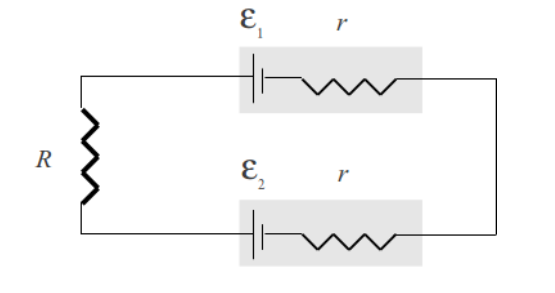
\includegraphics[width=0.4\textwidth]{hw5_p4_question.png}
		\end{center}
	\end{small}
\end{figure}

\begin{solution}
	\begin{enumerate}[(a)]
		\item Suppose there is a current flowing clockwise, whose magnitude is $i$. Then
		      \begin{align}
			                        & \varepsilon_1 + 2ir + iR - \varepsilon_2 = 0 \\
			      \Rightarrow \quad & i = -0.4\ [A]
		      \end{align}
		      Showing that the current is flowing counter-clockwise with magnitude of 0.4 $A$.
		\item The rate of dissipation of electrical energy is equal to the power of elements. Hence
		      \begin{align*}
			      P_R & = i^2 R = 1.28\ [W]  \\
			      P_r & = 2i^2 r = 0.32\ [W]
		      \end{align*}
		\item $\varepsilon_1$, $P_1 = 12 \times 0.4 = 4.8\ [J/s]$.
		\item $\varepsilon_2$, $P_2 = 8 \times 0.4 = 3.2\ [J/s]$.
		\item Notice that 
              \begin{align}
                P_R + P_r + P_2 = P_1
              \end{align}
              Namely, the rates of consumption and production are identical.
	\end{enumerate}

\end{solution}


\noindent\rule{7.1in}{2.8pt}

%%%%%%%%%%%%%%%%%%%%%%%%%%%%%%%%%%%%%%%%%%%%%%%%%%%%%%%%%%%%%%%%%%%%%%%%%%%%%%%%%%%%%%%%%%%%%%%%%%%%%%%%%%%%%%%%%%%%%%%%%%%%%%%%%%%%%%%%
% Problem 5
%%%%%%%%%%%%%%%%%%%%%%%%%%%%%%%%%%%%%%%%%%%%%%%%%%%%%%%%%%%%%%%%%%%%%%%%%%%%%%%%%%%%%%%%%%%%%%%%%%%%%%%%%%%%%%%%%%%%%%%%%%%%%%%%%%%%%%%%
\begin{problem}{5}{4}
\par For the circuit shown in the figure below, find the current through each of the resistors. For numerical calculations assume: $R_1=2\Omega$, $R_2=4\Omega$, $R_3=5\Omega$, $\varepsilon_1=20V$,
$\varepsilon_2=14V$, $\varepsilon_3=36V$. The internal resistance of the emfs is negligible.
\end{problem}
\begin{figure}[!htbp]
	\begin{small}
		\begin{center}
			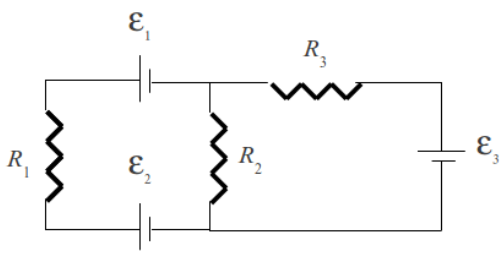
\includegraphics[width=0.4\textwidth]{hw5_p5_question.png}
		\end{center}
	\end{small}
\end{figure}

\begin{solution}
	\par Suppose the current in the left loop(mesh) is $i_1$, and the current in the right loop(mesh) is $i_2$. \\
	Then we have
	\begin{align}
		-\varepsilon_1 + i_1R_1 + \varepsilon_2 + (i_1-i_2)R_2 & = 0 \\
		-\varepsilon_3 + i_2R_3 + (i_2-i_1)R_2                  & = 0
	\end{align}
	Then we get
	\begin{align}
		\left\{
		\begin{array}{c}
			i_1 = \frac{99}{19}\ [A] \\
			i_2 = \frac{120}{19}\ [A]
		\end{array}
		\right.
	\end{align}
	Hence we know the current passing through each resistor.
	\begin{align}
		i_{R_1} = \frac{99}{19}\ [A] \qquad i_{R_2} = \frac{21}{19}\ [A] \qquad i_{R_3} = \frac{120}{99}\ [A]
	\end{align}
\end{solution}

\noindent\rule{7.1in}{2.8pt}

%%%%%%%%%%%%%%%%%%%%%%%%%%%%%%%%%%%%%%%%%%%%%%%%%%%%%%%%%%%%%%%%%%%%%%%%%%%%%%%%%%%%%%%%%%%%%%%%%%%%%%%%%%%%%%%%%%%%%%%%%%%%%%%%%%%%%%%%
% Problem 6
%%%%%%%%%%%%%%%%%%%%%%%%%%%%%%%%%%%%%%%%%%%%%%%%%%%%%%%%%%%%%%%%%%%%%%%%%%%%%%%%%%%%%%%%%%%%%%%%%%%%%%%%%%%%%%%%%%%%%%%%%%%%%%%%%%%%%%%%
\begin{problem}{6}{3}
\par For the circuit shown in the figure below what happens to the brightness
of the bulbs when the switch $S$ is closed if the battery (a) has no internal
resistance and (b) has non-negligible internal resistance? Explain why.
\end{problem}
\begin{figure}[!htbp]
	\begin{small}
		\begin{center}
			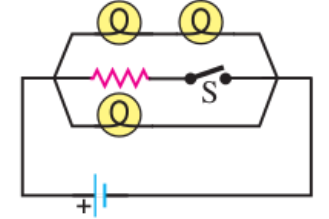
\includegraphics[width=0.2\textwidth]{hw5_p6_question.png}
		\end{center}
	\end{small}
\end{figure}

\begin{solution}
	\par For (a), the brightness of the bulb will not change since the voltage applied
	on the bulb has not changed. The \textbf{terminal voltage} is still equal to \textbf{emf}.
	\par For (b), the brightness of the bulb will decrease since the whole resistance of the
	system will decrease when the switch closed, thus the \textbf{terminal voltage} will decrease
	as well. Hence the brightness decreases.
\end{solution}

\noindent\rule{7.1in}{2.8pt}

%%%%%%%%%%%%%%%%%%%%%%%%%%%%%%%%%%%%%%%%%%%%%%%%%%%%%%%%%%%%%%%%%%%%%%%%%%%%%%%%%%%%%%%%%%%%%%%%%%%%%%%%%%%%%%%%%%%%%%%%%%%%%%%%%%%%%%%%
% Problem 7
%%%%%%%%%%%%%%%%%%%%%%%%%%%%%%%%%%%%%%%%%%%%%%%%%%%%%%%%%%%%%%%%%%%%%%%%%%%%%%%%%%%%%%%%%%%%%%%%%%%%%%%%%%%%%%%%%%%%%%%%%%%%%%%%%%%%%%%%
\begin{problem}{7}{4}
Four resistors are connected to form a Wheatstone bridge - a circuit that
can be used to measure unknown resistance $X$, provided the resistances of
$N$, $M$ and $P$ are known. The idea of the measurement method is to tune
(with the switches $K_1$ and $K_2$ closed) the variable resistance $M$ so that the
potential difference between points $b$ and $c$ is zero and the galvanometer
does not show any current. The bridge is then said to be balanced. Show
that in this configuration $X = MP/N$.
\end{problem}
\begin{figure}[!htbp]
	\begin{small}
		\begin{center}
			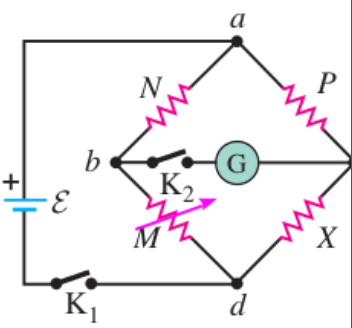
\includegraphics[width=0.2\textwidth]{hw5_p7_question.png}
		\end{center}
	\end{small}
\end{figure}

\begin{solution}
	Suppose the current flowing in \texttt{a-b-d} is $i_1$ while the current flowing
	in \texttt{a-c-d} is $i_2$. Then according to KVL
	\begin{align}
		i_1(N+M) - i_2(P+X) = 0 \\
	\end{align}
	According to the balance condition
	\begin{align}
		\varepsilon - i_1N = \varepsilon - i_2P
	\end{align}
	Hence
	\begin{align*}
		\frac{N}{P} = \frac{i_2}{i_1} = \frac{N+M}{P+X}
	\end{align*}
	Hence
	\begin{align*}
		\frac{N}{P} = \frac{M}{X}
	\end{align*}
	Namely
	\begin{align}
		X = \frac{MP}{N}
	\end{align}
\end{solution}

\noindent\rule{7.1in}{2.8pt}

%%%%%%%%%%%%%%%%%%%%%%%%%%%%%%%%%%%%%%%%%%%%%%%%%%%%%%%%%%%%%%%%%%%%%%%%%%%%%%%%%%%%%%%%%%%%%%%%%%%%%%%%%%%%%%%%%%%%%%%%%%%%%%%%%%%%%%%%
% Problem 8
%%%%%%%%%%%%%%%%%%%%%%%%%%%%%%%%%%%%%%%%%%%%%%%%%%%%%%%%%%%%%%%%%%%%%%%%%%%%%%%%%%%%%%%%%%%%%%%%%%%%%%%%%%%%%%%%%%%%%%%%%%%%%%%%%%%%%%%%
\begin{problem}{8}{3}
Strictly speaking, the formula $q(t)=Q_{\max } e^{-t / R C}$ implies that an infinite amount of time is required to discharge a capacitor
in a $R-C$ circuit completely. Yet for practical purposes, a capacitor may be considered to be fully discharged after a finite time
$t_{\mathrm{d}}$, defined as the time when the charge on the capacitor $q\left(t_{\mathrm{d}}\right)$ differs from zero by no more than
the charge of one electron.
\begin{enumerate}[(a)]
	\item Find $t_{\mathrm{d}}$ if $C=0.92 \mu \mathrm{F}, R=670 \mathrm{k} \Omega$, and $Q_{\max }=7 \mu \mathrm{C}$.
	\item For a given $Q_{\max }$ is the time required to reach this state always the same number of time constants, independent of $R$ and $C .$ Why or why not?
\end{enumerate}
\end{problem}

\begin{solution}
	\begin{enumerate}[(a)]
		\item Plug in the data
		      \begin{align*}
			                        & q_e = Q_{max}^{-\frac{t_d}{RC}} \\
			      \Rightarrow \quad & t_d = 19.36\ [s]
		      \end{align*}
		\item Based on (a)
		      \begin{align}
			      \ln\left( \frac{q_e}{Q_{max}} \right) = -\frac{t_d}{RC}
		      \end{align}
		      Hence we conclude that, $t_d$ does not depend on $R$ or $C$ separately but
		      depend on $RC$ as a whole. Namely, if $RC$ is constant, $t_d$ is also a constant.
	\end{enumerate}

\end{solution}

\end{document}